\section{Experiment Setup Details}
\label{app:exp_details}

This section provides a detailed breakdown of the datasets and hyperparameters used in our experiments. All experiments were conducted on a cluster of NVIDIA H200 GPUs.

\subsection{Dataset Details}
\label{app:datasets}
Our training was conducted on a curated mathematics dataset. For evaluation, especially for analyzing generalization (as mentioned in the main text), we utilized a comprehensive suite of benchmarks spanning multiple domains. The composition of this evaluation suite is detailed in Table~\ref{tab:eval_suite_appendix}.

\begin{table*}[t]
\centering
\begin{tabular}{lrll}
\toprule
\textbf{Dataset} & \textbf{Samples} & \textbf{Huggingface Tag} & \textbf{Domain} \\
\midrule
Held-out Data & 500 & LLM360/guru-RL-92k & Math \\
aime2024 & 30 & Maxwell-Jia/AIME\_2024 & Math \\
amc2023 & 40 & knoveleng/AMC-23 & Math \\
codegen\_humaneval & 164 & openai/openai\_humaneval & Code \\
gsm8k & 1319 & openai/gsm8k & Math \\
logic\_zebra\_puzzle & 200 & LLM360/guru-RL-92k & Logical Reasoning \\
math & 500 & HuggingFaceH4/MATH-500 & Math \\
stem\_supergpqa & 200 & LLM360/guru-RL-92k & STEM \\
\midrule
\textbf{Total} & \textbf{2953} & & \\
\bottomrule
\end{tabular}
\caption{Composition of the multi-domain evaluation suite.}
\label{tab:eval_suite_appendix}
\end{table*}

\subsection{Hyperparameter Configuration}
\label{app:hyperparams}
All experiments were conducted with a consistent set of hyperparameters for the Group Relative Policy Optimization (GRPO) algorithm to ensure a fair comparison across different model sizes and configurations. The key hyperparameters are listed in Table~\ref{tab:hyperparams_appendix}.

\begin{table}[H]
\centering
\begin{tabular}{ll}
\toprule
\textbf{Hyperparameter} & \textbf{Value} \\
\midrule
Learning Rate & $1e-6$ \\
Batch Size & 512 \\
KL Loss Coefficient & 0.001 \\
Rollout Temperature (Training) & 1.0 \\
Rollout Temperature (Evaluation) & 0.7 \\
Clip Ratio (High \& Low) & 0.2 \\
Input Sequence Length & 2048 \\
Output Sequence Length & 4096 \\
\bottomrule
\end{tabular}
\caption{GRPO training hyperparameters used across all experiments.}
\label{tab:hyperparams_appendix}
\end{table}

\subsection{Prompt Templates}
\label{app:prompts}
This section details the specific prompt templates used for evaluating models on different domains. For each task, the model was provided with the corresponding instruction prepended to the problem statement \texttt{<question>}. Check the details in Table~\ref{tab:prompt_templates}.
\begin{table*}[tb]
\centering
\begin{tabular}{>{\raggedright\arraybackslash}p{3cm} >{\raggedright\arraybackslash}p{\dimexpr\linewidth-3cm-2\tabcolsep\relax}}
\toprule
\textbf{Domain} & \textbf{Prompt Template} \\
\midrule
Mathematics & \texttt{You are a knowledgeable math assistant. Answer the following questions and think step by step\textbackslash{}n<question>\textbackslash{}nPlease output the final answer within \textbackslash{}\textbackslash{}boxed\{\}.} \\
\midrule
Code & \texttt{Write a complete, self-contained Python solution to the following problem. Your solution must include all necessary imports and the full function definition, including the signature exactly as specified. Do not modify the function signature or docstring.\textbackslash{}n<question>} \\
\midrule
Logic & \texttt{Solve the following puzzle\textbackslash{}n<question>\textbackslash{}nPlease return the final answer in <answer> </answer> tags, for example <answer> \{"header": ["Position", "Nationality", "Job"], "rows": [["1", "british", "plumber"], ["2", "polish", "carpenter"]]\} </answer>.}  \\
\midrule
Science (STEM) & \texttt{You are a knowledgeable assistant. Answer the following questions and think step by step \textbackslash{}n <question> \textbackslash{}n put your final answer option within \textbackslash{}\textbackslash{}boxed\{\}. Only put the letter in the box, e.g. \textbackslash{}\textbackslash{}boxed\{A\}. There is only one correct answer} \\
\midrule
\end{tabular}
\caption{Prompt templates used for different evaluation domains.}
\label{tab:prompt_templates}
\end{table*}

\subsection{Data Reuse Experiment Setup}
\label{app:data-reuse-detailed}

\begin{figure}{H}
    \centering
    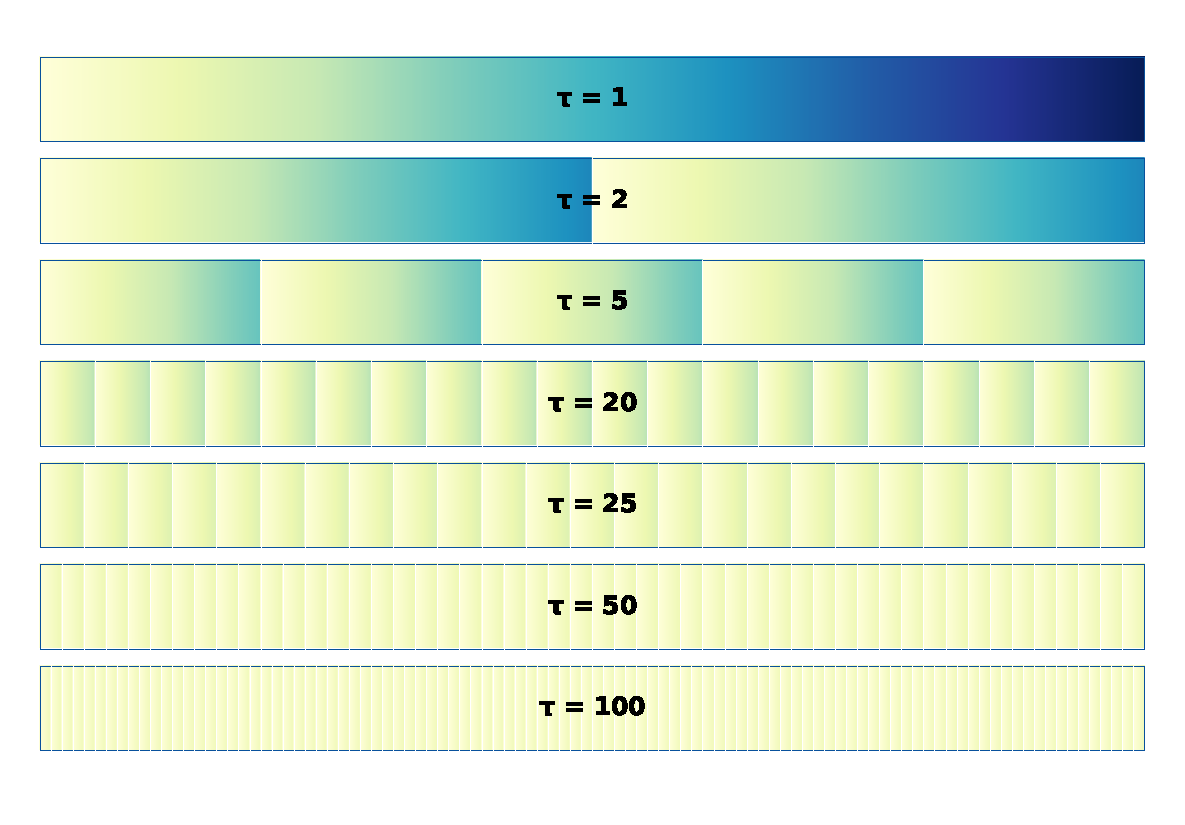
\includegraphics[width=0.95\linewidth]{./figures/datareuse/exp2_tau_rectangles.pdf}
    \caption{Data Reuse Schema}
    \label{fig:data_reuse_schematic}
\end{figure}

To systematically evaluate the effect of data reuse under constrained data scenarios, we design controlled experiments where all runs are trained with the same total data size but different levels of data repetition. Each run randomly samples a subset from the full training corpus and repeats this subset sufficiently many times to exactly match the target data budget (i.e., $\text{subset size} \times \tau = \text{total data size}$). Unlike \cite{muennighoff2023scaling}, subsets are sampled independently for each run rather than sampling within the larger subsets, to mitigate sampling bias and balance stochasticity across conditions. To remain consistent with the Curriculum Learning setting of the main experiments, examples within each subset are ordered by increasing difficulty; across epochs, this difficulty schedule is preserved and repeated rather than reshuffled, as illustrated in Figure~\ref{fig:data_reuse_schematic}. We also put the results for instruct model in Figure~\ref{fig:data_reuse_instruct}.
\begin{figure}[H]
    \centering
    % Placeholder: Instruct model's Final Loss vs. Data Reuse Factor
    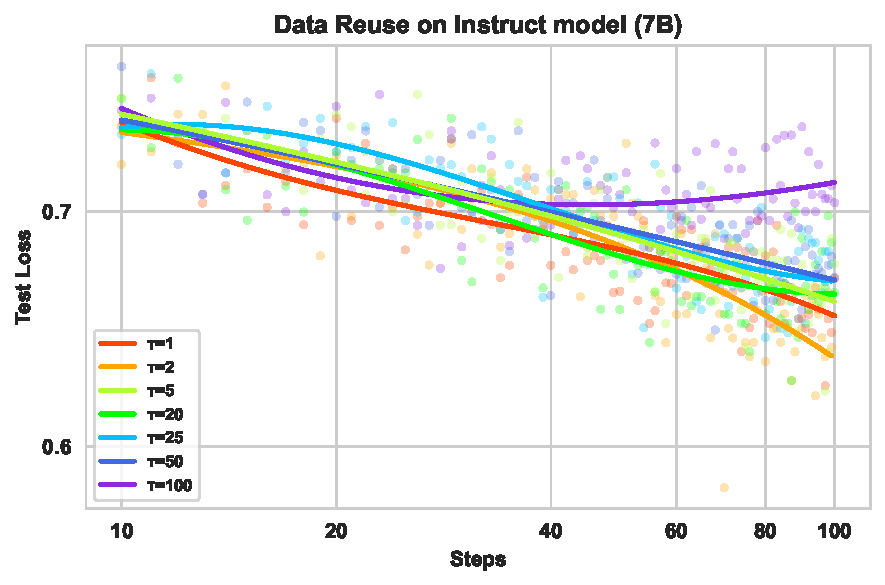
\includegraphics[width=\linewidth]{./figures/datareuse/fit_exp2-instruct_holdout_Tau_step_ErrRate.pdf}
    \caption{Instruct Model}
    \label{fig:data_reuse_instruct}
\end{figure}
% \subsection{Prompt Templates}
% \label{app:prompts}
% This section details the specific prompt templates used for evaluating models on different domains. For each task, the model was provided with the corresponding instruction prepended to the problem statement $<question>$.

% \begin{table}[H]
% \centering
% \caption{Prompt templates used for different evaluation domains.}
% \label{tab:prompt_templates}
% \begin{tabular}{ll}{>{\raggedright\arraybackslash}p{0.15\textwidth} >{\raggedright\arraybackslash}p{0.75\textwidth}}
% \toprule
% \textbf{Domain} & \textbf{Prompt Template} \\
% \midrule
% Mathematics & \texttt{You are a knowledgeable math assistant. Answer the following questions and think step by step\textbackslash{}n<question>\textbackslash{}nPlease output the final answer within \textbackslash{}\textbackslash{}boxed\{\}.} \\
% \midrule
% Code & \texttt{Write a complete, self-contained Python solution to the following problem. Your solution must include all necessary imports and the full function definition including the signature exactly as specified. Do not modify the function signature or docstring.\textbackslash{}n<question>} \\
% \midrule
% Logic & \texttt{Solve the following puzzle\textbackslash{}n<question>\textbackslash{}nPlease return the final answer in <answer> </answer> tags, for example <answer> \{"header": ["Position", "Nationality", "Job"], "rows": [["1", "british", "plumber"], ["2", "polish", "carpenter"]]\}} </answer>. \\
% \midrule
% Science (STEM) & \texttt{You are a knowledgeable assistant. Answer the following questions and think step by step\textbackslash{}n<question>\textbackslash{}nput your final answer option within \textbackslash{}\textbackslash{}boxed\{\}. Only put the letter in the box, e.g. \textbackslash{}\textbackslash{}boxed\{A\}. There is only one correct answer} \\
% \bottomrule
% \end{tabular}
% \end{table}
% \begin{figure*}[t]
%   \centering
%   \begin{subfigure}[t]{0.5\textwidth}
%     \centering
%     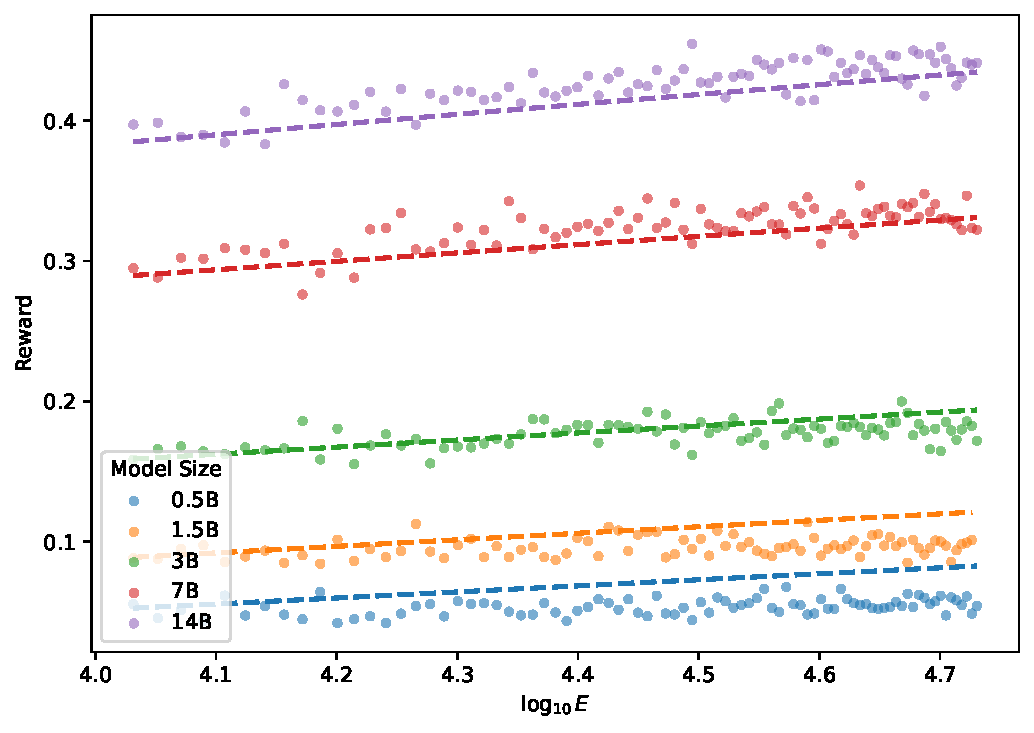
\includegraphics[width=\linewidth]{./figures/fit/holdout_fit_Reward_logE.pdf}
%     \caption{Fitted Data size (log) — Reward}
%   \end{subfigure}\hfill
%   \begin{subfigure}[t]{0.5\textwidth}
%     \centering
%     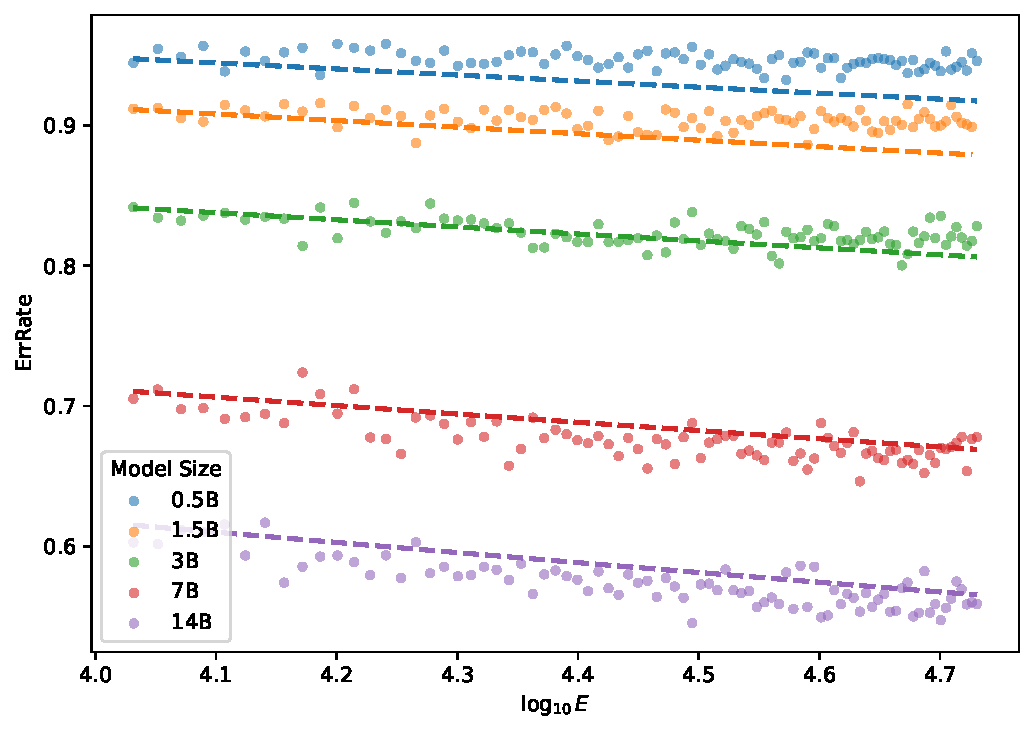
\includegraphics[width=\linewidth]{./figures/fit/holdout_fit_ErrRate_logE.pdf}
%     \caption{Fitted Data size (log) — Error Rate}
%   \end{subfigure}\hfill
% \end{figure*}